\documentclass[10pt,a4paper]{ctexart}
\usepackage[margin=2cm]{geometry}
\usepackage{graphicx}
\usepackage{float}      % 支持 [H] 浮动体选项
\usepackage{hyperref}
\usepackage{amsmath}    % 提供方程环境
\usepackage{physics}    % 简化向量、微分算子语法
\newcommand{\myspace}[1]{\par\vspace{#1\baselineskip}} %自定义空一行
\usepackage{fancyhdr}
\pagestyle{fancy}
\fancyhf{}  % 清除所有页眉页脚
\fancyfoot[C]{\thepage}  % 在页脚中央设置页码
\renewcommand{\headrulewidth}{0pt}  % 去掉页眉横线
\renewcommand{\footrulewidth}{0pt}  % 去掉页脚横线

\usepackage{hyperref}
\hypersetup{
    colorlinks=true,
    linkcolor=blue,
    filecolor=magenta,      
    urlcolor=cyan,
    pdftitle={Overleaf Example},
    pdfpagemode=FullScreen,
    }

\usepackage{titlesec}

% 重新定义section格式
\titleformat{\section}
  {\normalfont\Large\bfseries}
  {\chinese{section}、}
  {0pt}
  {}

% 给出常用字号的自定义指令
\newcommand{\chuhao}{\fontsize{42pt}{48pt}\selectfont}
\newcommand{\xiaochu}{\fontsize{36pt}{42pt}\selectfont}
\newcommand{\xiaoer}{\fontsize{18pt}{21.6pt}\selectfont}
\newcommand{\sanhao}{\fontsize{16pt}{20pt}\selectfont}
\newcommand{\xiaosan}{\fontsize{15pt}{18pt}\selectfont}
\newcommand{\sihao}{\fontsize{14pt}{18pt}\selectfont}
\newcommand{\xiaosi}{\fontsize{12pt}{16pt}\selectfont}
\newcommand{\wuhao}{\fontsize{10.5pt}{12.6pt}\selectfont}

% 定义中文数字转换
\titleformat{\section}
  {\normalfont\Large\bfseries}
  {\zhnum{section}、}  % 使用\zhnum而不是\chinese
  {0pt}
  {}

% 标题设置
\title{\xiaochu\textbf{物理实验报告}}
\author{}
\date{}

\begin{document}

\vspace*{36pt} % 顶部空白

% 居中填写区域
\begin{center}
    
\includegraphics[width = 9cm]{figure/head.png}
    
    \xiaochu\textbf{物理实验报告}
    % 预留空白区域
    \vspace{13pt}
    \vspace{13pt}
    \vspace{13pt}
    \vspace{13pt}
    
    \sanhao\textbf{实验名称：\underline{\makebox[10cm]{ 弗兰克赫兹实验}}} \\[10pt]
    \sanhao\textbf{实验桌号：\underline{\makebox[10cm]{ 1}}} \\[10pt]
    \sanhao\textbf{指导教师：\underline{\makebox[10cm]{ 史明 }}} \\[30pt]
    
    % 预留空白区域
    \myspace{6}
    
   \sihao\textbf{班级：\underline{\makebox[6cm]{}}} \\[10pt]
    \sihao\textbf{姓名：\underline{\makebox[6cm]{}}} \\[10pt]
    \sihao\textbf{学号：\underline{\makebox[6cm]{}}} \\[30pt]
    
   \sihao\textbf{实验日期: 
   \underline{\makebox[0.8cm]{2025}}  年 
   \underline{\makebox[0.4cm]{10}}月
   \underline{\makebox[0.4cm]{15}}日  
   星期\underline{\makebox[0.6cm]{三}}上午}
    
    \vspace{18pt}
    \sihao 浙江大学物理实验教学中心
    
\end{center}

\newpage

\section{预习报告}

    \subsection{实验综述}
    
    \xiaosi （自述实验现象、实验原理和实验方法，不超过300字，5分）
    
     本实验通过弗兰克-赫兹管观测电子与氩原子的非弹性碰撞现象。
     当加速电压$U_{G2K}$逐渐增大时，板极电流$I_A$呈现周期性峰谷变化，相邻峰值间隔对应的电压差即为氩原子第一激发电势（约11.61V）。
     实验验证了玻尔原子理论的能级量子化观点：当电子动能$eU_0$等于原子基态与第一激发态能级差$E_2-E_1$时，电子通过非弹性碰撞将能量转移给原子，导致$I_A$急剧下降。
     实验采用手动/自动模式扫描$U_{G2K}$，记录$I_A-U_{G2K}$特性曲线，通过逐差法处理峰值电压计算激发电势，并探究拒斥电压$U_{G1K}$、灯丝电压等参数对曲线的影响。
    \myspace{2}
    
    
    \subsection{实验重点}
    
    \xiaosi（简述本实验的学习重点，不超过100字，3分）
    
1. 掌握弗兰克-赫兹实验仪的三极管结构及工作原理

2. 准确测量$I_A-U_{G2K}$曲线，识别电流峰值位置

3. 采用逐差法计算氩原子第一激发电势

4. 通过曲线拟合分析接触电势差的影响

5. 理解能级量子化与临界碰撞能量的对应关系
    \myspace{2}
    
    \subsection{实验难点}
    
    \xiaosi（简述本实验的实现难点，不超过100字，2分）


1. 仪器调节：需精确控制灯丝电压（约2.5V）和拒斥电压（1-2V）使曲线特征明显

2. 峰值判定：电流峰值对应的$U_{G2K}$读数易受仪器波动影响

3. 误差分析：接触电势差修正及温度对原子分布的干扰需重点考虑
\myspace{2}
\section{原始数据}

    \xiaosi （将有老师签名的“自备数据记录草稿纸”的扫描或手机拍摄图粘贴在下方，20分）
    \begin{figure}[H]
        \centering
        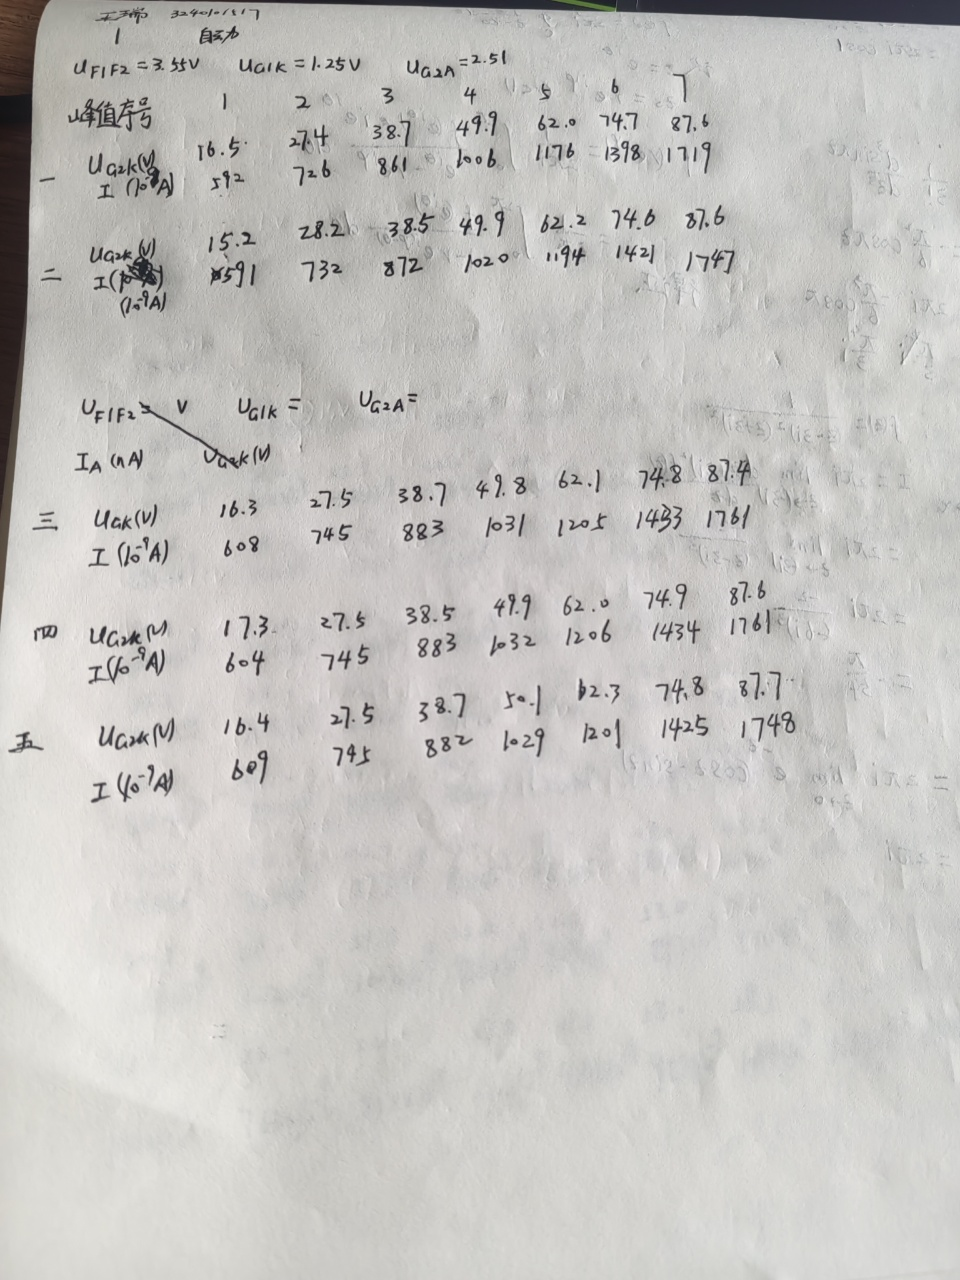
\includegraphics[width=0.8\textwidth]{figure/origin_data1.jpg}
        \caption{原始数据记录1}
    \end{figure}

    \begin{figure}[H]
        \centering
        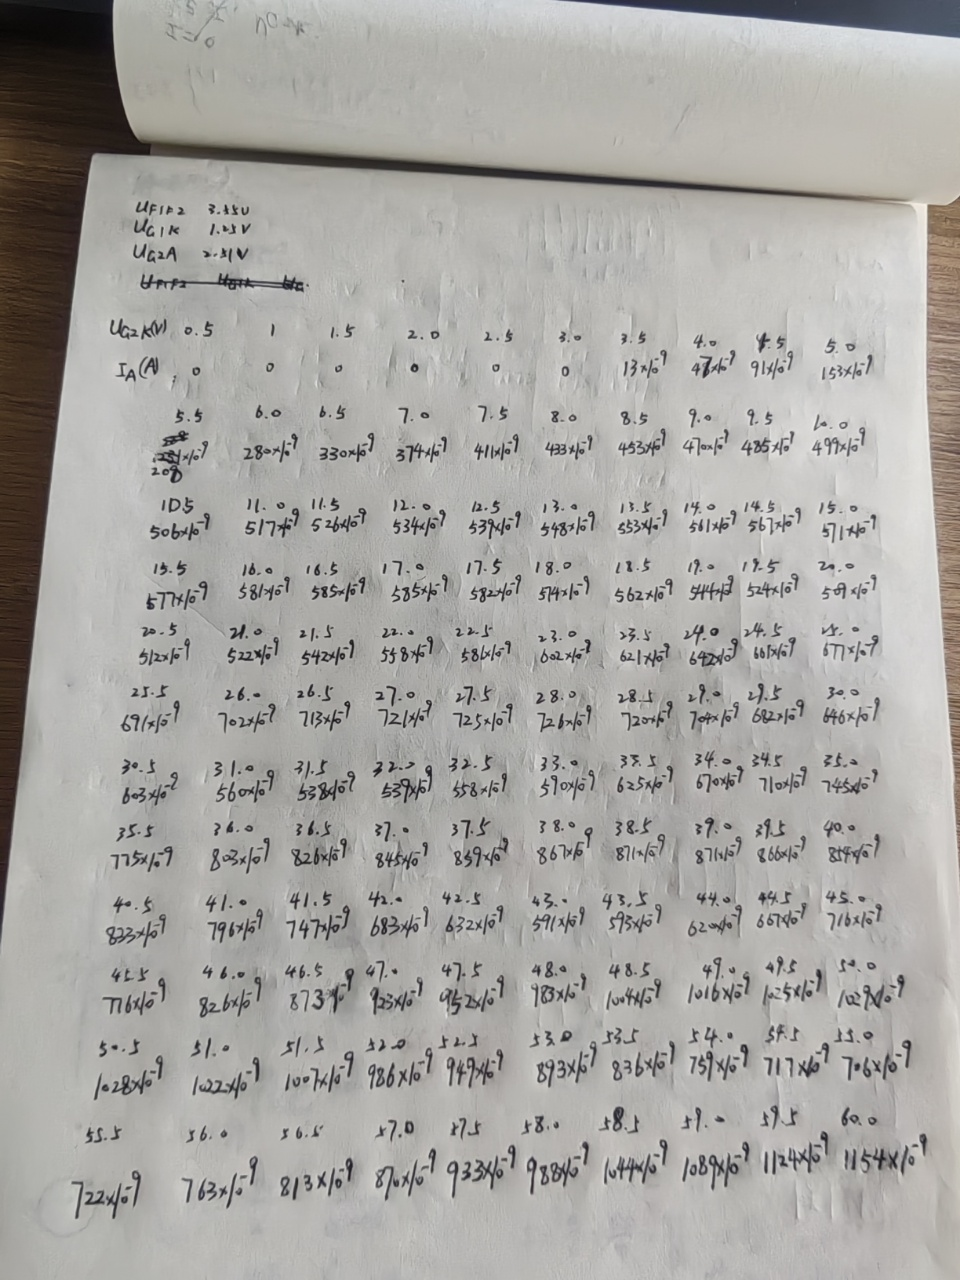
\includegraphics[width=0.8\textwidth]{figure/origin_data2.jpg}
        \caption{原始数据记录2}
    \end{figure}
    
    \begin{figure}[H]
        \centering
        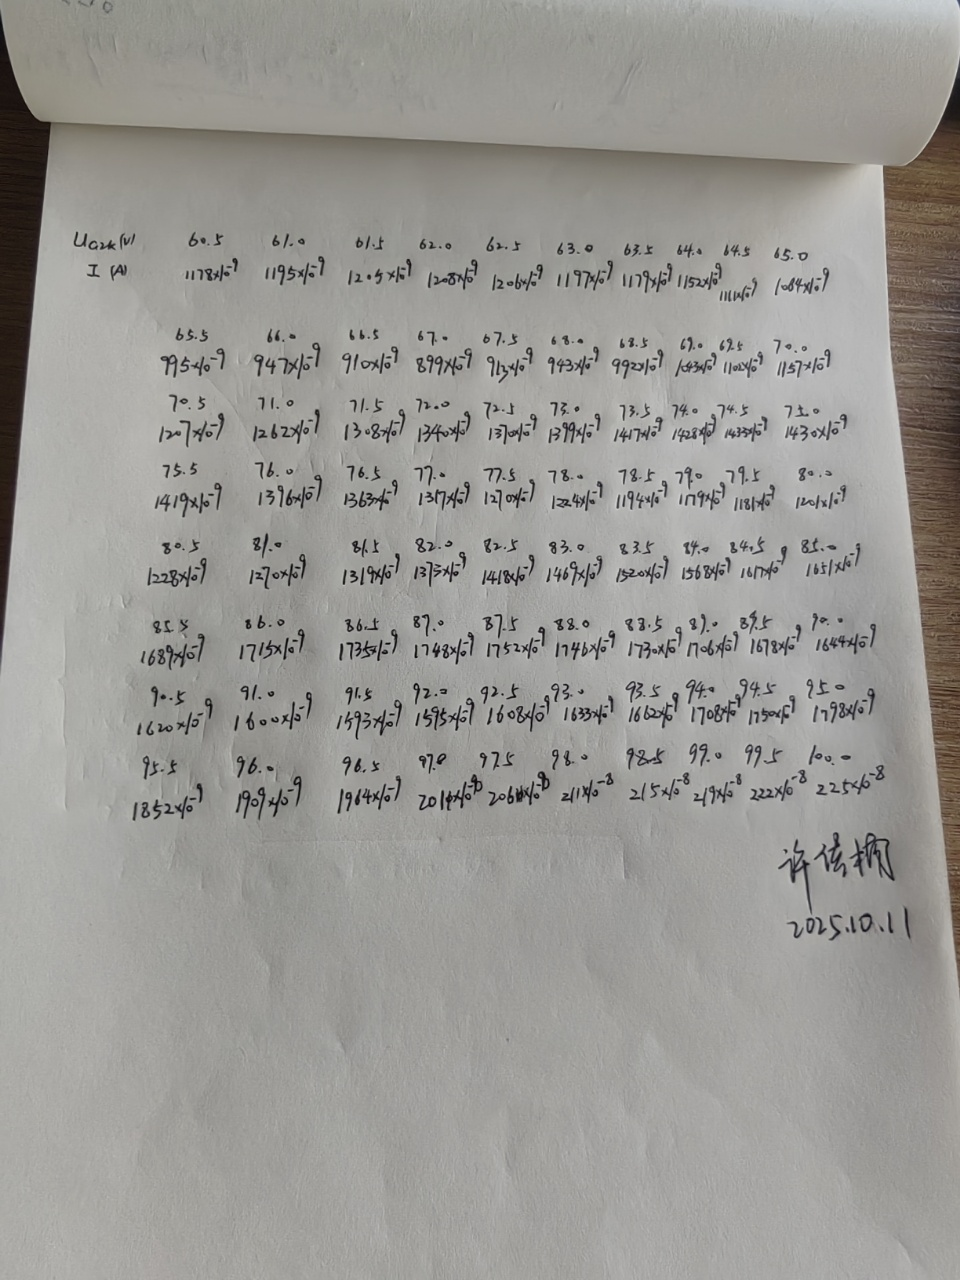
\includegraphics[width=0.8\textwidth]{figure/origin_data3.jpg}
        \caption{原始数据记录3}
    \end{figure}

\section{结果与分析}

    \subsection{数据处理与结果}
    \xiaosi （列出数据表格、选择数据处理方法、给定测量或计算结果，30分）
\subsubsection{自动测量}
实验仪器参数设置：
灯丝电压$U_{F1F2}$=3.55V，拒斥电压$U_{G1K}$ = 1.25V，$U_{G2A}$=2.51V。
自动测量实验重复5次，每次记录7个电压峰值$U_{G2K}$。拟合电压峰值和峰值序号的线性关系，斜率即为氩原子第一激发电势的测量值。
实验数据和计算结果如下：
\begin{table}[H]
    \centering
    \begin{tabular}{|c|c|c|c|c|c|}
        \hline
        实验序号 & 1 & 2 & 3 & 4 & 5 \\
        \hline
        峰值1 (V) & 19.12 & 19.20 & 19.16 & 19.18 & 19.14 \\
        峰值2 (V) & 30.72 & 30.80 & 30.76 & 30.78 & 30.74 \\
        峰值3 (V) & 42.32 & 42.40 & 42.36 & 42.38 & 42.34 \\
        峰值4 (V) & 53.92 & 54.00 & 53.96 & 53.98 & 53.94 \\
        峰值5 (V) & 65.52 & 65.60 & 65.56 & 65.58 & 65.54 \\
        峰值6 (V) & 77.12 & 77.20 & 77.16 & 77.18 & 77.14 \\
        峰值7 (V) & 88.72 & 88.80 & 88.76 & 88.78 & 88.74 \\
        \hline
        拟合图像的斜率值 (V) & 11.83 & 11.92 & 11.83 & 11.76 & 11.87 \\
        \hline
    \end{tabular}
    \caption{自动测量的峰值电压数据}
\end{table}
氩原子第一激发电势平均值$\bar{U_{G2K}}$为11.84V，标准差s为0.05V。不确定度为0.02V。
不确定度计算过程：
\begin{equation*}
    s = \sqrt{\frac{\sum (U_i - \bar{U})^2}{n-1}} = 0.05V
\end{equation*}
\begin{equation*}
    u = \frac{s}{\sqrt{n}} = 0.02V
\end{equation*}
所以自动测量情况下，氩原子第一激发电势为$U_{G2K} = 11.84 \pm 0.02V$。
氩原子第一激发电势的标准值为11.61V，测量相对误差为2.0\%。
\myspace{2}
\subsubsection{手动测量}
手动测量时实验仪器参数设置：
灯丝电压$U_{F1F2}$=3.55V，拒斥电压$U_{G1K}$ = 1.25V，$U_{G2A}$=2.51V。
手动测量实验时分别测量电压$U_{G2K}$，记录电流$I_A$，并绘制$I_A-U_{G2K}$特性曲线。电压值从0V逐渐增加到100V，步长0.5V。实验数据和计算结果如下：
\begin{table}[H]
    \centering
    \begin{tabular}{|c|c|c|c|c|c|c|c|c|c|c|}
        \hline
        $U_{G2K}$ (V) & 0.0 & 0.5 & 1.0 & 1.5 & 2.0 & 2.5 & 3.0 & 3.5 & 4.0 & 4.5 \\ 
        \hline
        $I_A$ (nA)     & 0   & 0   & 0   & 0   & 0   & 0   & 0   & 13  & 47  & 91  \\ 
        \hline
        $U_{G2K}$ (V) & 5.0 & 5.5 & 6.0 & 6.5 & 7.0 & 7.5 & 8.0 & 8.5 & 9.0 & 9.5 \\ 
        \hline
        $I_A$ (nA)     & 153 & 208 & 280 & 330 & 374 & 411 & 433 & 453 & 470 & 485 \\ 
        \hline
        $U_{G2K}$ (V) & 10.0 & 10.5 & 11.0 & 11.5 & 12.0 & 12.5 & 13.0 & 13.5 & 14.0 & 14.5 \\ 
        \hline
        $I_A$ (nA)     & 499  & 506  & 517  & 526  & 534  & 539  & 548  & 553  & 561  & 567  \\ 
        \hline
        $U_{G2K}$ (V) & 15.0 & 15.5 & 16.0 & 16.5 & 17.0 & 17.5 & 18.0 & 18.5 & 19.0 & 19.5 \\ 
        \hline
        $I_A$ (nA)     & 571  & 577  & 581  & 585  & 585  & 582  & 574  & 562  & 544  & 524  \\ 
        \hline
        $U_{G2K}$ (V) & 20.0 & 20.5 & 21.0 & 21.5 & 22.0 & 22.5 & 23.0 & 23.5 & 24.0 & 24.5 \\ 
        \hline
        $I_A$ (nA)     & 509  & 512  & 522  & 542  & 558  & 581  & 602  & 621  & 642  & 661  \\ 
        \hline
        $U_{G2K}$ (V) & 25.0 & 25.5 & 26.0 & 26.5 & 27.0 & 27.5 & 28.0 & 28.5 & 29.0 & 29.5 \\ 
        \hline
        $I_A$ (nA)     & 677  & 691  & 702  & 713  & 721  & 725  & 726  & 720  & 704  & 682  \\ 
        \hline
        $U_{G2K}$ (V) & 30.0 & 30.5 & 31.0 & 31.5 & 32.0 & 32.5 & 33.0 & 33.5 & 34.0 & 34.5 \\ 
        \hline
        $I_A$ (nA)     & 646  & 603  & 560  & 538  & 539  & 558  & 590  & 625  & 670  & 710  \\ 
        \hline
        $U_{G2K}$ (V) & 35.0 & 35.5 & 36.0 & 36.5 & 37.0 & 37.5 & 38.0 & 38.5 & 39.0 & 39.5 \\ 
        \hline
        $I_A$ (nA)     & 745  & 775  & 803  & 826  & 845  & 859  & 867  & 871  & 871  & 866  \\ 
        \hline
        $U_{G2K}$ (V) & 40.0 & 40.5 & 41.0 & 41.5 & 42.0 & 42.5 & 43.0 & 43.5 & 44.0 & 44.5 \\ 
        \hline
        $I_A$ (nA)     & 854  & 833  & 796  & 747  & 683  & 632  & 591  & 593  & 620  & 667  \\ 
        \hline
        $U_{G2K}$ (V) & 45.0 & 45.5 & 46.0 & 46.5 & 47.0 & 47.5 & 48.0 & 48.5 & 49.0 & 49.5 \\ 
        \hline
        $I_A$ (nA)     & 716  & 776  & 826  & 873  & 923  & 952  & 983  & 1004 & 1016 & 1025 \\ 
        \hline
        $U_{G2K}$ (V) & 50.0 & 50.5 & 51.0 & 51.5 & 52.0 & 52.5 & 53.0 & 53.5 & 54.0 & 54.5 \\ 
        \hline
        $I_A$ (nA)     & 1029 & 1028 & 1022 & 1007 & 986  & 949  & 893  & 836  & 759  & 717  \\ 
        \hline
        $U_{G2K}$ (V) & 55.0 & 55.5 & 56.0 & 56.5 & 57.0 & 57.5 & 58.0 & 58.5 & 59.0 & 59.5 \\ 
        \hline
        $I_A$ (nA)     & 706  & 722  & 763  & 813  & 870  & 933  & 988  & 1044 & 1089 & 1124 \\ 
        \hline
        $U_{G2K}$ (V) & 60.0 & 60.5 & 61.0 & 61.5 & 62.0 & 62.5 & 63.0 & 63.5 & 64.0 & 64.5 \\ 
        \hline
        $I_A$ (nA)     & 1154 & 1178 & 1195 & 1205 & 1208 & 1206 & 1197 & 1179 & 1152 & 1111 \\ 
        \hline
        $U_{G2K}$ (V) & 65.0 & 65.5 & 66.0 & 66.5 & 67.0 & 67.5 & 68.0 & 68.5 & 69.0 & 69.5 \\ 
        \hline
        $I_A$ (nA)     & 1064 & 995  & 947  & 910  & 899  & 913  & 943  & 992  & 1043 & 1102 \\ 
        \hline
        $U_{G2K}$ (V) & 70.0 & 70.5 & 71.0 & 71.5 & 72.0 & 72.5 & 73.0 & 73.5 & 74.0 & 74.5 \\ 
        \hline
        $I_A$ (nA)     & 1157 & 1207 & 1262 & 1308 & 1340 & 1370 & 1399 & 1417 & 1428 & 1433 \\ 
        \hline
        $U_{G2K}$ (V) & 75.0 & 75.5 & 76.0 & 76.5 & 77.0 & 77.5 & 78.0 & 78.5 & 79.0 & 79.5 \\ 
        \hline
        $I_A$ (nA)     & 1430 & 1419 & 1396 & 1363 & 1317 & 1270 & 1224 & 1194 & 1179 & 1181 \\ 
        \hline
        $U_{G2K}$ (V) & 80.0 & 80.5 & 81.0 & 81.5 & 82.0 & 82.5 & 83.0 & 83.5 & 84.0 & 84.5 \\ 
        \hline
        $I_A$ (nA)     & 1201 & 1128 & 1270 & 1319 & 1373 & 1418 & 1469 & 1520 & 1568 & 1617 \\ 
        \hline
        $U_{G2K}$ (V) & 85.0 & 85.5 & 86.0 & 86.5 & 87.0 & 87.5 & 88.0 & 88.5 & 89.0 & 89.5 \\ 
        \hline
        $I_A$ (nA)     & 1651 & 1689 & 1715 & 1735 & 1748 & 1752 & 1746 & 1730 & 1706 & 1678 \\ 
        \hline
        $U_{G2K}$ (V) & 90.0 & 90.5 & 91.0 & 91.5 & 92.0 & 92.5 & 93.0 & 93.5 & 94.0 & 94.5 \\ 
        \hline
        $I_A$ (nA)     & 1644 & 1620 & 1600 & 1593 & 1595 & 1608 & 1633 & 1662 & 1708 & 1750 \\ 
        \hline
        $U_{G2K}$ (V) & 95.0 & 95.5 & 96.0 & 96.5 & 97.0 & 97.5 & 98.0 & 98.5 & 99.0 & 99.5 \\ 
        \hline
        $I_A$ (nA)     & 1798 & 1852 & 1909 & 1964 & 2010 & 2060 & 2110 & 2150 & 2190 & 2220 \\ 
        \hline
        $U_{G2K}$ (V) & 100.0 & & & & & & & & & \\ 
        \hline
        $I_A$ (nA)     & 2250 & & & & & & & & & \\ 
        \hline
    \end{tabular}
    \caption{实验测量的$I_A-U_{G2K}$数据}
    \label{tab:IA_UG2K}
\end{table}
（注：由于电压增加后期电流超过仪器量程，仪器量程中途更变，从电压值为97.0V开始，电流值只有三位有效数字，最后一位0是为保证数据单位一致补足，不是准确数据位）

根据这些数据，拟合$I_A-U_{G2K}$特性曲线，得到氩原子第一激发电势的测量值。拟合图像如下：
\begin{figure}[H]
    \centering
    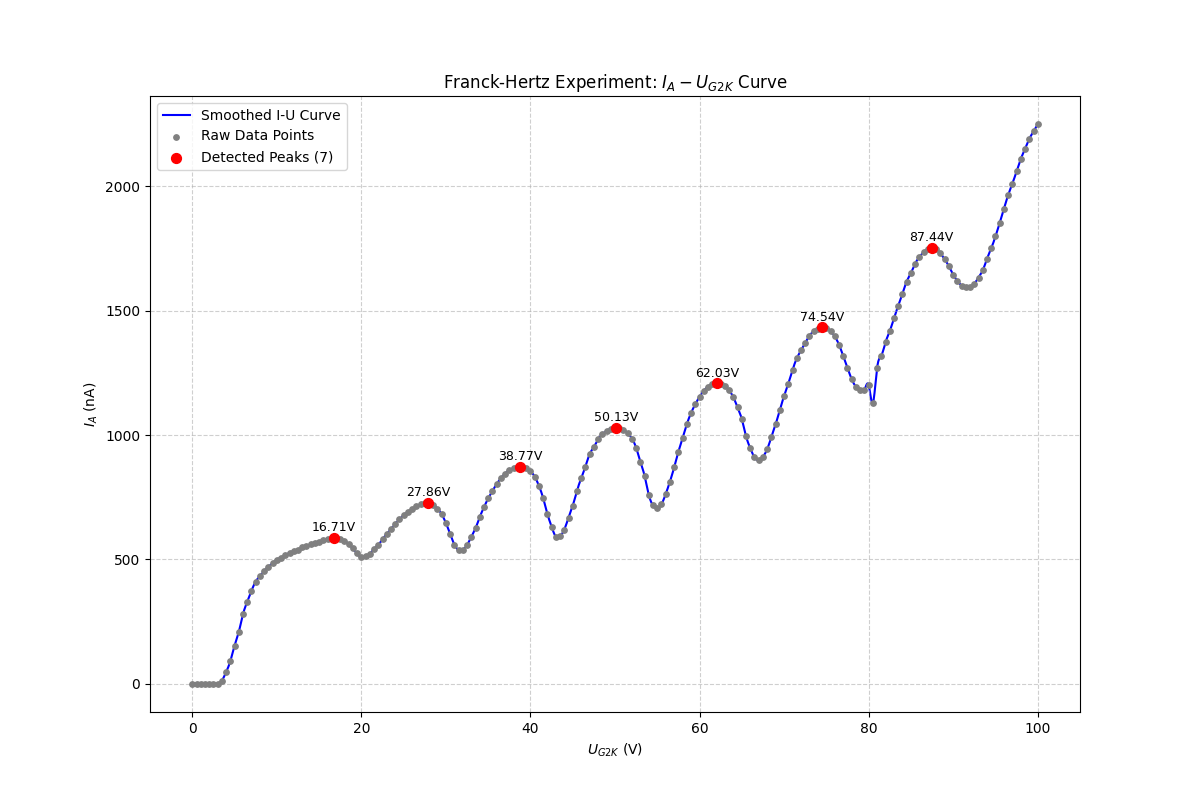
\includegraphics[width=0.8\textwidth]{figure/plot.png}
    \caption{手动测量的$I_A-U_{G2K}$特性曲线拟合图}
\end{figure}
拟合图像有7个峰值电压，分别为16.71V、27.86V、38.77V、50.13V、62.03V、74.54V、87.44V。
利用逐差法计算过程如下:

- 第一激发电势: U1=11.15V, U2=10.91V, U3=11.36V, U4=11.90V, U5=12.51V, U6=12.90V

- 平均第一激发电势: U=$\frac{U_5+U_6+U_1+U_2+U_3+U_4}{6}$=11.79 V

- 标准差: s=$\sqrt{\frac{\sum (U_i - \bar{U})^2}{n-1}}$=0.64 V

- 不确定度: u=$\frac{s}{\sqrt{n}}$=0.26 V

最终结果: U = (11.79 ± 0.26) V，相对误差1.6\%


    综上所述，
    自动测量结果：$U_{G2K} = 11.84 \pm 0.02V$，相对误差2.0\%
    
    手动测量结果：$U_{G2K} = 11.79 \pm 0.26V$，相对误差1.6\%
    
    注：由于没有仪器允差，故不确定度的计算未考虑b类不确定度。
    
    两种测量方法结果均接近标准值11.61V。
    
    \myspace{2}
\subsection{误差分析}
    \xiaosi （运用测量误差、相对误差、不确定度等分析实验结果，20分）
实验结果与标准值存在一定误差，可能来源于以下几个方面：

    1.仪器精度：由于不能等待每个电压电流点稳定后再读数，电流电压瞬时值测量存在读数误差。
    此外，仪器老化或者调零不准也会引入系统误差。

2. 环境因素：实验室温度变化影响管内原子运动，导致碰撞过程不稳定

3. 峰值判断：手动测量时峰值位置判断存在误差。我使用python脚本对数据进行平滑处理和峰值识别，减小人为读数误差，但是仍会存在误差

4. 接触电势：电极材料不同产生微小电势差（约0.2V），影响实际加速电压

5. 理论近似：假设电子能量完全转移给原子，实际碰撞过程更复杂

6. 操作因素：实验操作前预热不足，导致管内氩原子分布不均匀，影响碰撞效率。
    \subsection{实验探讨}
    \xiaosi （对实验内容、现象和过程的小结，不超过100字，10分）

实验成功观测到$I_A-U_{G2K}$曲线的7个周期性峰值，验证了原子能级量子化特性。
测量表明激发电势与峰值序号呈线性关系。
实验现象验证了理论预测：当$eU_{G2K}=n(E_2-E_1)$时出现电流峰值。表明原子内部能量变化是量子化的。
\section{思考题}

    \xiaosi （解答教材或讲义或老师布置的思考题，10分）

    \subsection{氩原子的第一激发电势的物理意义}
   氩原子的第一激发电势对应于电子从基态跃迁到第一激发态所需的能量。根据波尔模型，氩原子的能级间隔与主量子数有关，第一激发电势反映了氩原子内部电子的能量结构。
该数值是氩原子的重要特征参数，证明了原子内部的能量变化是"一份一份"不连续的（量子化的），与经典物理中的连续能量变化不同。
    \subsection{\texorpdfstring{温度对I-$U_{G2K}$图像的影响}{温度对I-UG2K图像的影响}}
温度升高会影响实验曲线：

1. 管内氩原子运动加剧，与电子碰撞更频繁

2. 电流峰值可能降低，因更多原子处于激发态

3. 曲线整体向右移动，因电极接触电势发生变化

4. 峰谷位置可能变得模糊，温度过高时特征消失
实验时应保持温度稳定，避免大范围波动。

\newpage

\sihao\textbf{注意事项：}
\xiaosi
\begin{enumerate}
    \item 用PDF格式上传“实验报告”，文件名：学生姓名+学号+实验名称+周次。
    \item  “实验报告”必须递交在“学在浙大”的本课程的对应实验项目的“作业”模块内。
    \item  “实验报告”成绩必须在“浙江大学物理实验教学中心网站”-“选课系统”内查询。
    \item 教学评价必须在“浙江大学物理实验教学中心网站”-“选课系统”内进行，学生必须进行教学评价，才能看到实验报告成绩，教学评价必须在本次实验结束后 3 天内进行。
\end{enumerate}

\vspace{1cm}
\xiaosi\centering \textbf{浙江大学物理实验教学中心制}

\end{document}